\documentclass[10pt]{article}

\usepackage{graphicx}
\usepackage{amsmath,amssymb}
\usepackage{gensymb}
\usepackage{mathtools}
\usepackage{etoolbox}
\usepackage{booktabs}
\usepackage{float}
\usepackage{graphicx}
\usepackage{geometry}
\usepackage{multicol}
\usepackage{caption}

\newcommand\mgin{0.5in}
\geometry{
	left=\mgin,
	right=\mgin,
	bottom=\mgin,
	top=\mgin
}

% Set path to import figures from
\graphicspath{{../figures/}}

% Place converted graphics in current directory
\usepackage[outdir=./]{epstopdf}

% Define multicolumn figure-like environment
% from http://tex.stackexchange.com/questions/12262/multicol-and-figures
\newenvironment{mcfig}
	{\par\medskip\noindent\minipage{\linewidth}}
	{\endminipage\par\medskip}

% Define error function for math mode
\newcommand{\erf}{\mbox{erf}}
% Sign function
\newcommand{\sign}{\mbox{sign}}
% Real numbers
\newcommand\R{\mathbb{R}}
% Norm
\newcommand\norm[1]{||#1||}
% Length matrix entries
\newcommand\LL{\mathcal{L}}
% Frond population
\newcommand\FF{\mathcal{F}}

% arara: pdflatex

\begin{document}

%%fakesection Title
\null

\thispagestyle{empty}
\addtocounter{page}{-1}

\begin{center}
    \begin{sffamily}
	\begin{bfseries}
	    \null
	    \vfill
	    \Huge{A Kelp Farming Approach to Sustainable Wastewater Nutrient Removal and Bioenergy Production at Wastewater Treatment Plants with Ocean Outfalls} \\

	    \vspace{20pt}
	    \LARGE{Project Summary} \\
	    \vspace{20pt}
		\Large{ASSETs to Serve Humanity NSF REU 2016} \\
		\Large{Clarkson University} \\
	    \vspace{20pt}
    \begin{Large}
		Oliver Evans \\
		Dr. Shane Rogers \\
		Dr. Ole Jacob Broch \\
	\vspace{20pt}
	\today \\
    \end{Large}
	\end{bfseries}
    \end{sffamily}
    \vspace{30pt}

    \null
    \vfill
    \vfill
    \null
\end{center}
\pagebreak


% Increase table cell height (not for header)
\renewcommand{\arraystretch}{1.5}

\begin{multicols}{2}

\section{Introduction}
I spent this summer participating in an REU at Clarkson University developing a mathematical model for the light field in a macroalgae aquaculture environment. The impetus for this project was as follows: Dr. Rogers was approached by the operator of a wastewater treatment plant in Boothbay Harbor, Maine, who is facing increasingly demanding EPA regulations limiting the concentration of certain nutrients permissible to be released into the ocean via wastewater treatment outfalls.
In order to adhere to these stricter requirements using conventional nutrient remediation, a significant quantity of specialized equipment would be necessary, which is not currently present in the Boothbay Harbor plant.
Being surrounded on all sides by water and private property, the treatment plant lacks the necessary space for the additional equipment, and would therefore need to move their entire facility to a new location in order to conform to these new nutrient regulations.

As an alternative to conventional nutrient remediation techniques, Dr. Rogers has proposed the cultivation of the macroalgae \textit{Saccharina Latissima} (sugar kelp) near the outfall site.
The purpose of such an undertaking would be twofold: to prevent eutrophication of the surrounding ecosystem by sequestering the nutrients in question, and to reduce one of the primary expenses in macroalgae cultivation: nutrient input.
Once grown, a variety of products can be derived from macroalgae, including biofuel, fish/cattle feedstock, and high value chemical materials such as alginate and agar.
Food for human consumption is also a common product of kelp aquaculture, though it may not be ideal for a wastewater treatment application.

Thus, we seek to investigate the feasibility, and optimal implementation of kelp farming in wastewater treatment operations. 
Specifically, I seek to develop an accurate model of the light field in a kelp farming environment as a function of both the spacing and depth of the kelp plants, and of the quality of the water itself.
Ole Jacob Broch is a mathematician at SINTEF, a research organization in Trondheim, Norway, who has been working to model the growth of \textit{Saccharina Latissima} using SINMOD, a large-scale 3D hydrodynamical ocean model developed at SINTEF.
Ultimately, my aim is that my light model can be used both independently and in conjunction with Dr. Broch's SINMOD model.

\section{Physical Setup}
Being a salt water species, macroalgae cultivation occurs primarily in the ocean, with the exception of the initial stage of growth, where microscopic kelp spores are inoculated onto a thread in a small laboratory pool.
This thread is then wrapped around a large rope, which is placed in the ocean and generally suspended by buoys in one of two configurations: horizontal or vertical.
Thus far, I am primarily concerned with modeling the vertical rope case, in which the kelp plants extend radially outward from the rope in all directions, which are made up of a single frond (leaf), stipe (stem) and holdfast (root structure).
We consider a rectangular grid of such vertical ropes. 
Plants extending from each rope will shade both themselves and their neighbors to varying degrees based on the depth of the kelp, the rope spacing, the angle of incident light and the nature of scattering in the water.
In addition, light will be naturally absorbed by the water to varying degrees as determined by the clarity of the water.

\begin{mcfig}
	\centering
	\includegraphics[width=3.5in]{kelp_array}
	\captionof{figure}{$4\times 4$ array of vertical kelp ropes}
\end{mcfig}
\section{Coordinate System}
For all of our three dimensional analysis, we will use the absolute coordinate system defined in figure \ref{fig:3dcoords}.
In the following sections, we will wish to convert between Cartesian and spherical coordinates, which we will do using the following formulas.
\begin{align}
	\begin{split}
		x & = r\sin\phi\cos\theta \\
		y & = r\sin\phi\sin\theta \\
		z & = r\cos\phi \\
	\label{eqn:coords}
	\end{split}
\end{align}

Therefore, for some function $f(x,y,z)$, we can write its derivative along a path in spherical coordinates in terms of Cartesian coordinates using the chain rule.
\begin{equation}
	\frac{\partial f}{\partial r} 
	=\frac{\partial f}{\partial x}\frac{\partial x}{\partial r} 
	+ \frac{\partial f}{\partial y}\frac{\partial y}{\partial r} 
	+ \frac{\partial f}{\partial z}\frac{\partial z}{\partial r}
\end{equation}
Then, calculating derivatives from \eqref{eqn:coords}, we get
\begin{equation}
	\frac{\partial f}{\partial r} 
	=\frac{\partial f}{\partial x}r\sin\phi\cos\theta
	+ \frac{\partial f}{\partial y}r\sin\phi\sin\theta
	+ \frac{\partial f}{\partial z}r\cos\phi
	\label{eqn:partials}
\end{equation}
\begin{figure}[H]
	\centering
	\includegraphics[width=3in]{3d_coords}
	\caption{Downward-facing right-handed coordinate system with radial distance $r$ from the origin, distance $s$ from the $z$ axis, zenith angle $\phi$ and azimuthal angle $\theta$}
	\label{fig:3dcoords}
\end{figure}

\section{Notation and Discretization}
In this model, we discretize several quantities, though we also make statements about their continuous behavior.
We also use information about a quantity related to an individual in order to draw conclusions about the distribution over the whole population.
It will therefore be necessary to interchange between discrete and continuous notation, so it will be helpful to be clear upfront about our use of symbols.
Note that not all of this notation will apply to every quantity.

Let $x$ be some quantity which we seek to quantify.
Then the value of this quantity for a single individual will be denoted by $x$ (lowercase letter).
This is the continuous variable over which we might integrate a continuous function of the quantity.

The partition values which we choose in order to discretize this quantity will be denoted $x_i$ (lowercase letter with subscript).
Since all of our partitions will be uniform, let we denote the width of our partition on $x$ by $h_x$, where $h_x>0$.
That is, $x_{i+1} - x_i = h_x \forall i = 1,\ldots,n_x$, where $n_x$ is the size of our partition.
Furthermore, denote the minimum partition value by $m_x$ and the maximum by $M_x$.
Then $M_x - m_x = nh_x$.

The normalized continuous distribution among the whole population will be denoted by $X$ (capital letter) such that $\int_a^bX(x)\,dx$ is the proportion of the population whose $x$ values are between $a$ and $b$.
Finally, the population proportion in a discrete bin determined by the chosen partition on $x$ will be denoted by $X_i$ (capital letter with subscript).
That is, $X_i = \int_{x_i}^{x_{i+1}}X(x)\,dx$.

Specifically, let the following quantities be discretized in this way on the respective intervals.

\begin{mcfig}
	\centering
	\begin{tabular}{ccl} \toprule
		$x$ & $[m_x,M_x]$ & description \\
		\midrule
		$x$ & $[m_x,M_x]$ & horizontal distance \\
		$y$ & $[m_y,M_y]$ & horizontal distance \\
		$z$ & $[0,M_z]$ & depth \\
		$t$ & $[0,M_t]$ & time \\
		$l$ & $[0,M_l]$ & frond length \\
		$\theta_f$ & $[-\pi,\pi]$ & frond angle \\
		$\theta$ & $[-\pi,\pi]$ & azimuth angle \\
		$\phi$ & $[0,\pi]$ & polar angle \\
		\bottomrule \\
	\end{tabular}
	\captionof{figure}{Discretized quantities}
\end{mcfig}

In some cases, it will also be convenient to specify the individual whose quantity value we are considering.
In this case, given an individual $f$ in the population, we represent the $x$ value of $f$ by $f(x)$.

\section{Population Distribution}
\label{sec:dist}
\subsection{Frond angle distribution}
\label{sec:angle_dist}
The frond angle varies according to the von Mises distribution, which is the periodic analogue of the normal distribution.
It is defined on $[-\pi,\pi]$ rather than $(-\infty,\infty)$.
It has two parameters, $\mu$ and $\kappa$, which shift and sharpen the distribution respectively.
%$\kappa$ can be considered analogous to $1/\sigma$ in the normal distribution.
Here, we use $\mu = \theta_w$ and $\kappa = v_w$.

The PDF for this distribution is
\begin{equation}
	P_{\theta_f}(\theta_f) = \frac{e^{(v_w)\cos(\theta_f-v_w)}}{2\pi I_0(v_w)}
\end{equation}
where $I_0(x)$ is the modified Bessel function of the first kind of order 0.
Notice that unlike the normal distribution, the von Mises distribution approaches a \textit{non-zero} uniform distribution as $\kappa$ approaches 0.
\begin{equation}
	\displaystyle \lim_{v_w \to 0}P_{\theta_f}(\theta_f) = \frac{1}{2\pi} \;\forall\, \theta_f \in [-\pi,\pi]
\end{equation}
The idea behind using this distribution is that with zero current velocity, the frond angles should be distributed uniformly, while as current velocity increases, they should be increasingly likely to be pointing in the direction of the current.
Note that $\theta_w$ and $v_w$ are functions of position.
For a given depth layer, we will use the average water velocity for that depth.

\begin{mcfig}
	\centering
	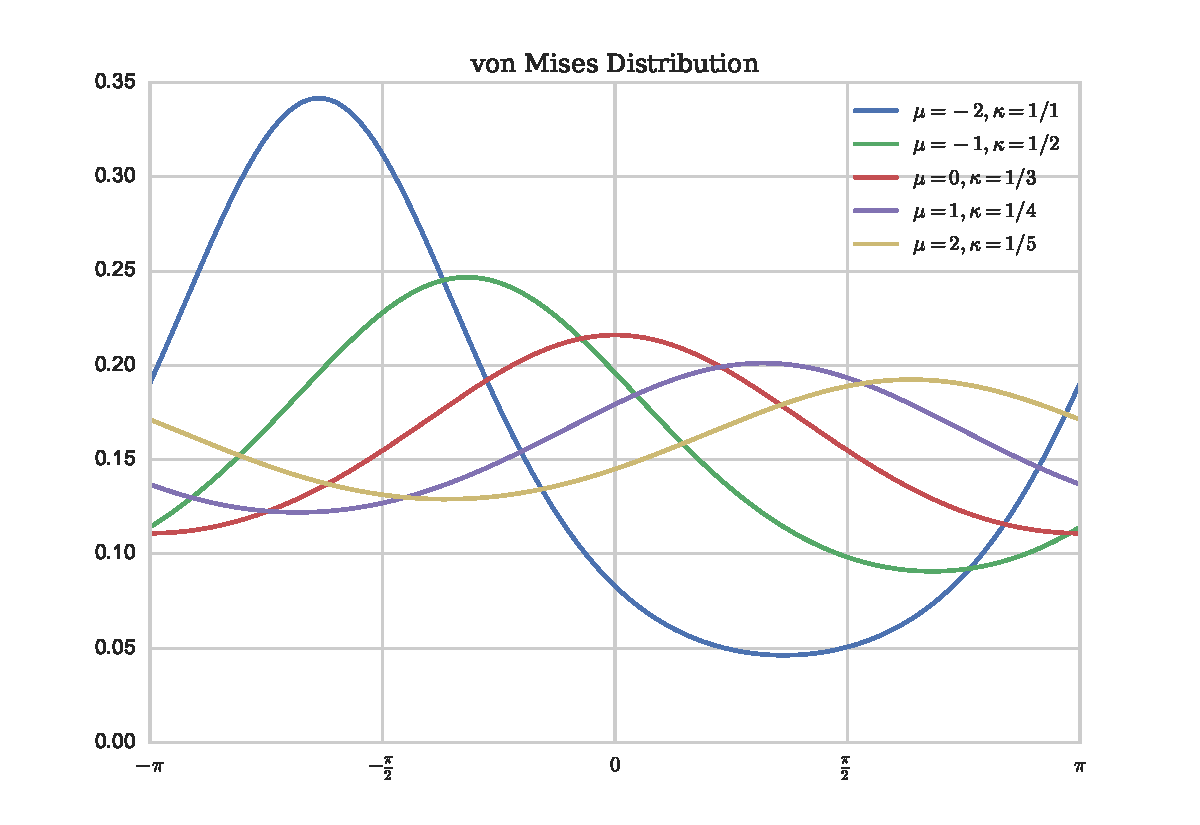
\includegraphics[width=\linewidth]{vonmises_2}
	\captionof{figure}{von Mises distribution for a variety of parameters}
	\label{fig:vonmises}
\end{mcfig}

\subsection{Length Distribution}
Consider the subpopulation $S_k$ of fronds which lies in the depth interval $z \in [z_k,z_{k+1})$.
Let the proportion of this subpopulation whose length is in the interval $l \in [l_i,l_{i+1})$ at time $t_n$ be denoted by $\LL_{k,i}^n$.

That is,
\begin{equation}
	\LL_{k,i}^n = \frac{\displaystyle\int_{z_k}^{z_{k+1}}\int_{l_i}^{l_{i+1}}L(l,z)\,dl\,dz}
	{\displaystyle\int_{z_k}^{z_{k+1}}\int_0^\infty L(l,z)\,dl\,dz}
	\label{eqn:lmatrix}
\end{equation}

for $i=1,\ldots,n-1$ and $k=1,\ldots,n$ where $L_k(l)$ is the length distribution of the subpopulation $S_k$.
Note that we define $\LL_{k,i}^n$ for $i=M_l$ in the same manner except that the length integral on this final column runs from $l_{M_l} \to \infty$. That is, the final column also includes any kelp fronds which may have outgrown the simulation parameters.
Of course, $M_l$ would ideally be chosen large enough such that it is an upper bound on frond lengths at all times.

Let the matrix $\LL^n = \left(\LL_{k,i}^n\right)$ be called the \textit{length matrix} at time $t_n$.
Calculating the change of the length matrix over time is our primary interest in this simulation.


\subsection{Combined 2D length-angle distribution}
\label{sec:2d_dist}
The previous two distributions are independent of one another. That is, the angle of the frond does not depend on the length, or vice versa.
Therefore, the probability of a frond simultaneously having a given frond length and angle is the product of their individual probabilities.

Given independent events $A$ and $B$,
\begin{equation}
	\label{eq:ind_prob}
	P(A \cap B) = P(A)P(B)
\end{equation}
Then the probability of frond length $l$ and frond angle $\theta_f$ coinciding is 
\begin{equation}
	P_{2D}(\theta_f,l) = P_{\theta_f}(\theta_f) \cdot L(l)
\end{equation}
A contour plot of this 2D distribution for a specific set of parameters is shown in figure \ref{fig:dist_2d}, where probability is represented by color in the 2D plane.
Darker green represents higher probability, while lighter beige represents lower probability.
In figure \ref{fig:kelp_sample}, 50 samples are drawn from this distribution and plotted.

It is important to note that if $P_{\theta_f}$ were dependent on $l$, the above definition of $P_{2D}$ would no longer be valid.
For example, it might be more realistic to say that larger fronds are less likely to bend towards the direction of the current.
In this case, \eqref{eq:ind_prob} would no longer hold, and it would be necessary to use the following more general relation.
\begin{equation}
	P(A \cap B) = P(A)P(B|A) = P(B)P(B|A)
\end{equation}
This is currently not taken into consideration in this model.

\begin{mcfig}
	\centering
	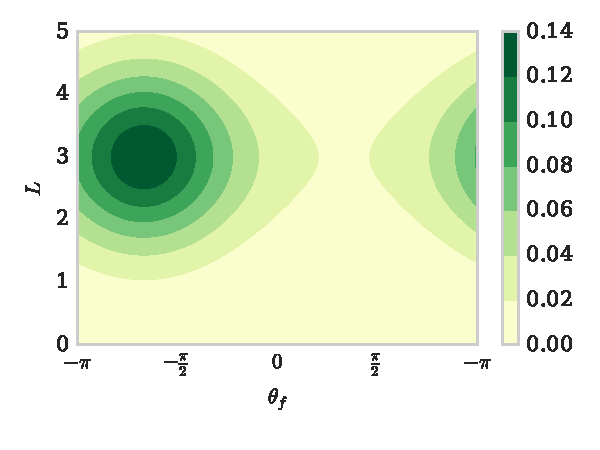
\includegraphics[width=\linewidth]{prob_2d}
	\vspace{-3em}
	\captionof{figure}{2D length-angle probability distribution with $\theta_w=2\pi/3,v_w=1$}
	\label{fig:dist_2d}
\end{mcfig}

\begin{mcfig}
	\centering
	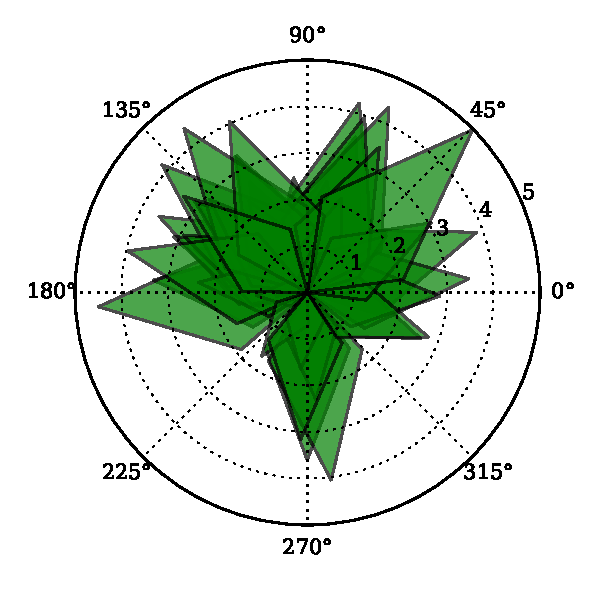
\includegraphics[width=\linewidth]{kelp_sample}
	\vspace{-2em}
	\captionof{figure}{A sample of 50 kelp fronds with length and angle picked from the distribution above with $f_s=0.5$ and $f_r=2$.}
	\label{fig:kelp_sample}
\end{mcfig}

\section{2D Model}
First, let us consider a 2D vertical slab of width $dz$ of a single rope with kelp extending from it.
We assume that the number (not mass) density of kelp plants, $\rho$ is initially uniform along the length of the rope.

\subsection{Frond shape}
\label{sec:shape}

\begin{mcfig}
	\centering
	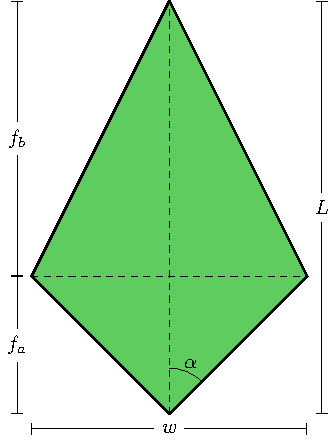
\includegraphics[width=2in]{frond}
	\captionof{figure}{Model frond diagram}
	\label{fig:frond}
\end{mcfig}

The frond is a kite with length $l$ from base to tip, and width $w$ from left to right.
 In figure \ref{fig:frond}, the base is shown at the bottom and the tip is shown at the top.
 The shortest distance from the base to the diagonal connecting the left and right corners is called $f_a$, and the shortest distance from that diagonal to the tip is called $f_b$.
 Clearly,
 \begin{equation}
	 f_a + f_b = l
 \end{equation}
When considering a whole population with varying sizes, it is more convent to specify ratios than absolute lengths.
Let the following ratios be defined.
\begin{align}
	f_r &= \frac{l}{w} \\
	f_s &= \frac{f_a}{f_b}
\end{align}
These ratios are assumed to be consistent among the entire population, making all fronds geometrically similar.
With these definitions, the shape of the frond can be fully specified by $l$, $f_r$, and $f_s$.
It is possible, then, to redefine $w$, $f_a$ and $f_b$ as follows from the preceding formulas.

\begin{align}
	w &= \frac{l}{f_r} \\
	f_a &= \frac{lf_s}{1+f_s} \\
	f_b &= \frac{l}{1+f_s}
\end{align}

The angle $\alpha$, half of the angle at the base corner, will be important in our analysis.
Using the above equations,
\begin{equation}
	\alpha = \tan^{-1}\left(\frac{2f_rf_s}{1+f_s}\right)
\end{equation}

\subsection{Relative coordinate system}
\label{sec:rel_coords}
To determine under what conditions a frond will shade a given point, we begin by describing the shape of the frond in Cartesian and then polar coordinates.
Of primary interest are the edges connected to the frond tip.
For convenience, we will use a relative coordinate system $(\theta',s)$ such that the line connecting the base to the tip is vertical, with the base at $(0,0)$.
The Cartesian analogue of this coordinate system, $(x',y')$, has the following properties.
\begin{align}
	x' &= s\cos\theta' \\ 
	y' &= s\sin\theta'
\end{align}
and
\begin{align}
	s &= \sqrt{x'^2+y'^2}
\end{align}
\vspace{-1em}
\begin{align}
	\theta' &= 
	\begin{cases}
		\tan^{-1}\left( \frac{y}{x} \right) & x > 0 \\
		\tan^{-1}\left( \frac{y}{x} \right) + \pi & x < 0 \\
		\frac{\pi}{2} & x = 0, y > 0 \\
		-\frac{\pi}{2} & x = 0, y < 0 \\
	\end{cases}
\end{align}


\subsection{Variables and functions}
\begin{mcfig}
	\centering
	\begin{tabular}{@{}llc@{}} \toprule
		symbol                    & description                           & model input \\ \midrule
		$l$                       & Frond length                          & \\
		$w$                       & Frond width                           & \\
		$f_a$                     & Inner frond length                    & \\
		$f_b$                     & Outer frond length                    & \\
		$\alpha$                  & Frond shape angle                     & \\
		$\theta_f$                & Frond direction angle                 & \\
		$f_s$                     & Frond shape parameter                 & \checkmark \\
		$f_r$                     & Frond length-width ratio              & \checkmark \\
		$v_w$                     & Water current speed                   & \checkmark \\
		$\theta_w$                & Water current angle                   & \checkmark \\
		$x,y$                     & Cartesian coordinates                 & \\
		$\theta,s$                & Polar coordinates                     & \\
		$t$                       & Time                                  & \\
		$P_{\theta_f}(\theta_f)$  & Frond angle PDF                       & \\
		$P_{2D}(\theta_f,l)$      & 2D length-angle distribution          & \\
		$S(\theta')$              & Angular sign function                 & \\
		$s_f(\theta)$             & Frond outer edge function             & \\ 
		$l_{min}(\theta)$         & Min. $l$ value to shade a point       & \\
		$R_s(\theta,s)$           & Shading region for a point            & \\
		$P_k(\theta,s)$           & Probability of kelp occupying a point & \\ 
		$R(x,y,z,\theta,\phi)$    & Radiance                              & \\
		$E(x,y,z)$                & Irradiance                            & \\
		$\tau,T_\theta$           & Frond transform                       & \\
		$W_\theta$                & 2D rotation matrix                    & \\
		$G(\Phi,l)$               & Growth function                       & \\
		$\LL_{i,k}^n$             & Length matrix                         & \\
		\bottomrule
	\end{tabular}
	\captionof{figure}{Model quantities. Those marked with a prime (e.g. $x'$) are relative to the frond, as described in section \ref{sec:rel_coords}.}
	\label{fig:variables}
\end{mcfig}

\subsection{Functional description of frond edge}
With this coordinate system established, we can describe the outer two edges of the frond in Cartesian coordinates as a piecewise linear function connecting the left corner: $(-w/2,f_a)$, the tip: $(0,l)$, and the right corner: $(w/2,f_a)$.
This function has the form
\begin{equation}
	y'_f(x') = l-\sign(x')\frac{f_b}{w/2}x'
\end{equation}
where
\begin{align}
	\sign(x) = 
	\begin{cases}
		1 & x > 0 \\
		0 & x = 0 \\
		-1 & x < 0 \\
	\end{cases}
\end{align}

Using the equations in section \ref{sec:rel_coords}, this can be written in polar coordinates after some rearrangement as
\begin{equation}
	s_f'(\theta') = \frac{l}{\sin\theta' + S(\theta')\frac{2f_b}{w}\cos\theta'}
\end{equation}
where
\begin{equation}
	S(\theta') = \sign(\theta'-\pi/2)
\end{equation}

Then, using the relationships in section \ref{sec:shape}, we can rewrite the above equation in terms of our frond ratios $f_s$ and $f_r$.
\begin{equation}
	\label{eq:rf_rel}
	s_f'(\theta') = \frac{l}{\sin\theta' + S(\theta')\frac{2f_r}{1+f_s}\cos\theta'}
\end{equation}

\subsection{Absolute coordinates}
\label{sec:abs_coords}
To generalize to a frond pointed at an angle $\theta_f$, we will use the coordinate system $(\theta,s)$ such that
\begin{equation}
	\theta = \theta' + \theta_f - \frac{\pi}{2}
\end{equation}
Then, for a frond pointed at the arbitrary angle $\theta_f$, the function for the outer edges can be written as 
\begin{equation}
	\label{eq:rf_abs}
	s_f(\theta) = s_f'\left(\theta - \theta_f + \frac{\pi}{2} \right)
\end{equation}

\subsection{Conditions for shading}
Consider a fixed frond of length $l$ at an angle $\theta_f$. In this section, we discuss ``shading'' in two dimensions. In this context, we say that a point $(\theta,s)$ is shaded by the frond if it lies within the region occupied by the frond. That is,
\begin{align}
	\left|\theta_f - \theta \right| < \alpha
	\shortintertext{and}
	s < s_f(\theta)
\end{align}

Equivalently, letting the point $(\theta,s)$ be fixed, a frond shades the point if the following conditions are satisfied.
\begin{align}
	\theta - \alpha < \theta_f < \theta + \alpha
	\label{eqn:rs_th}
	\shortintertext{and}
	l > l_{min}(\theta,s)
	\label{eqn:rs_l}
\end{align}
where
\begin{equation}
	l_{min}(\theta,s) = s \cdot \frac{l}{s_f(\theta)}
\end{equation}


Then, considering the point to be fixed, \eqref{eqn:rs_th} and \eqref{eqn:rs_l} define the spacial region $R_s(\theta,s)$ called the ``shading region for $(\theta,s)$'' with the property that if the tip of a frond lies within this region (i.e. $(\theta_f,l) \in R_s(\theta,s)$), then it shades the point.
$R_s(3\pi/4,3/2)$ is shown in blue in figure \ref{fig:shade_area} and the smallest possible shading fronds for several values of $\theta_f$ are shown in various colors.
Any frond longer than these at the same angle will also shade the point.

\begin{mcfig}
	\centering
	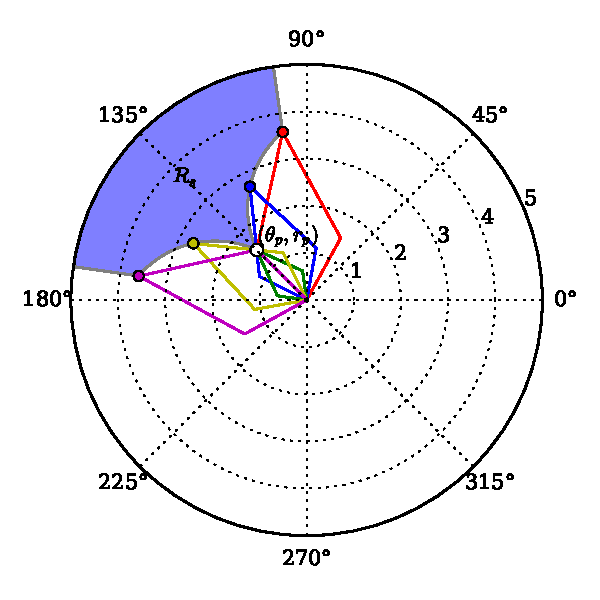
\includegraphics[width=\linewidth]{shade_area}
	\vspace{-2em}
	\captionof{figure}{Outlines of minimum-length fronds for a variety of angles to shade the point $(\theta,s)=(3\pi/4,3/2)$}
	\label{fig:shade_area}
\end{mcfig}

\subsection{Probability of shading}
We are interested in the probability that, given a fixed point $(\theta,s)$, values of $l$ and $\theta_f$ chosen from the distributions described in section \ref{sec:dist} will fall in the shading region.
This is found by integrating $P_{2D}$ over the shading region for $(\theta,s)$, as depicted in figure \ref{fig:cart_shade}.

\begin{mcfig}
	\centering
	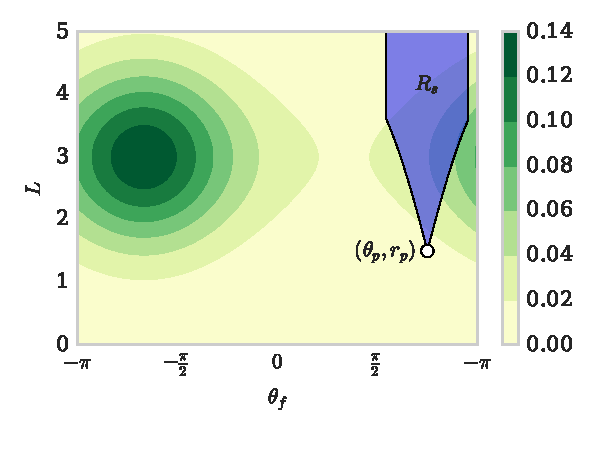
\includegraphics[width=\linewidth]{cart_shade}
	\vspace{-3em}
	\captionof{figure}{Contour plot of $P_{2D}(\theta_f,l)$ overlayed with the region in the $\theta_f-l$ plane which results in shading of the point $(\theta,s)=(3\pi/4,3/2)$}
	\label{fig:cart_shade}
\end{mcfig}

Now, we are able to define the probability of a frond occupying the point $(\theta,s)$ at a depth $z$ at time $t$ by
\begin{align}
		P_k(\theta,s,z,t)	&= \iint_{R_s(\theta,s,z,t)}
								P_{2D}(\theta_f,l)
								\;dl\;d\theta_f \nonumber \\
							&= \int_{\theta-\alpha}^{\theta+\alpha} 
								\int_{l_{min}(\theta_f,z,t)}^\infty
								P_{2D}(\theta_f,l)
								\;dl\;d\theta_f
\end{align}

\begin{mcfig}
	\centering
	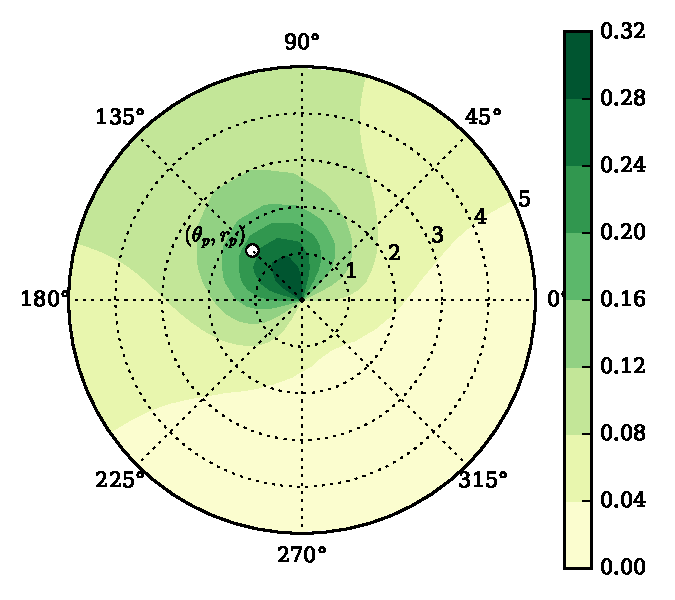
\includegraphics[width=\linewidth]{prob_shade}
	\vspace{-2em}
	\captionof{figure}{Contour plot of the probability of shading sampled at 121 points using $\theta_f=2\pi/3,v_w=1$}
	\label{fig:prob_shade}
\end{mcfig}

\section{Radiative Transfer Equation}
\subsection{Background}
In terms of optical quantities, our primary interest is in the radiance at each point from all directions, which affects the photosynthetic rate of the kelp, and therefore the total amount of biomass producible in a given area as well as the total nutrient absorption potential.
The equation governing the radiance throughout the system is known as the Radiative Transfer Equation (RTE), which has been largely unutilized in the fields of oceanography and aquaculture.
Meanwhile, it has been studied extensively in two fields: stellar astrophysics and computer graphics.
In its full form, radiance is a function of 3 spatial dimensions, 2 angular dimensions, and frequency, making for an incredibly complex problem.
Thus far, I have ignored the dependence on frequency, and have only considered monochromatic radiation.
The RTE states that along a given path, radiance is decreased by absorption and scattering out of the path, while it is increased by emission and scattering into the path.
In our situation, emission is negligible, owing only perhaps to some small luminescent phytoplankton or some such anomaly, and can therefore be safely ignored.
\subsection{Optical Definitions}
One of the most fundamental quantities in optics is radiant flux $\Phi$, which is the has units of energy per time.
The quantity of primary interest in modeling the light field is radiance $R$, which is defined as the radiant flux per steradian per projected surface area perpendicular to the direction of propagation of the beam.
That is,
\begin{equation}
	R = \frac{d^2\Phi}{dA d\omega}
\end{equation}
We must now define a few inherent optical properties (IOPs) which depend only on the medium of propagation.

Consider a beam of light traveling through the water in the direction $\underline{\omega} = (\theta,\phi)$.
As it travels, there will be some decrease in the radiance due to scattering and absorption.
Let $a_w$ and $b_w$ be the coefficients of absorption and scattering respectively due solely to the water.
Similarly, define $a_k$ and $b_k$ to be the absorption and scattering coefficients due solely to kelp.
The loss due to scattering or absorption, whether by kelp or water, is proportional to radiance, and $a_w,b_w,a_k,b_k$ all have units of inverse meters.

There will also be some gain into the path of the beam due to scattering from other directions, as determined by the \textit{volume scattering function},
$\displaystyle \beta(\Delta\theta): [0,\pi) \rightarrow \R^+$, which gives the proportion of incident radiance scattered at an angle $\Delta\theta$ from its original direction due to only water.
The units of $\beta$ are $\mbox{m}^{-1}\mbox{rad}^{-2}$.

For convenience, let $\displaystyle \beta(\underline{\omega}_1,\underline{\omega}_2) = \beta\left(\cos^{-1}\left(\frac{\underline{\omega}_1\cdot\underline{\omega}_2}{\norm{\underline{\omega}_1}\norm{\underline{\omega}_1}}\right)\right)$. 

\subsection{PDE}
From the discussion above, our governing PDE, the radiative transfer equation, can be written as
\begin{equation}
	\frac{\partial R}{\partial r} = 
	- c_kP_k - (1-P_k)c_w
	+ \iint_{4\pi}
	\beta_k(\underline{\omega},\underline{\omega}')
	R(x,y,z,\underline{\omega}')\,d\underline{\omega}'
	\label{eqn:rte1}
\end{equation}
where $c_k = a_k + b_k$, $c_w = a_w + b_w$, and $\underline{\omega}' \neq \underline{\omega}$.

Using \eqref{eqn:partials}, this can be rewritten in terms of Cartesian coordinates as
\begin{align}
	\begin{split}
	\frac{\partial R}{\partial x}\sin\phi \cos\theta 
	&+ \frac{\partial R}{\partial y}\sin\phi \sin\theta
	+ \frac{\partial R}{\partial z}\cos\phi \\ 
	&= - c_kP_k - (1-P_k)c_w \\
	&+ \iint_{4\pi}
	\beta_k(\underline{\omega},\underline{\omega}')
	R(x,y,z,\underline{\omega}')\,d\underline{\omega}'
	\end{split}
	\label{eqn:rte2}
\end{align}
\subsection{Boundary Conditions}
Though I have determined the PDE which governs the behavior of the radiance in the domain, I am lacking a full set of appropriate boundary conditions for the system.

Since we have one derivative per spatial dimension, we need one boundary condition per spatial dimension as well.
For $x$ and $y$, it may be favorable to use periodic boundary conditions in order to simulate a large array of kelp ropes spread out over the surface of the ocean.
It is worth mentioning, though, that special consideration may be necessary in order to account for smaller rope grids, for which edge effects neglected by periodic boundary conditions may become relevant.

It is the $z$ boundary condition which is puzzling me.
We should be able to make reasonable assumptions about the incident radiation from the atmosphere, though it seems that this is not sufficient.
We can only use atmospheric conditions for downwelling radiation.
It doesn't seem reasonable that radiance from above would have a direct effect on upwelling radiation.
In this sense, we only have half of the boundary condition that we need.
Then it seems that the other half should come from the bottom of the simulation.
But I would like to avoid putting any kind of specifically reflective or absorptive boundary on the \textit{bottom} of the simulation box, since the ocean would likely be much larger than the kelp.
In this case, it would be of interest to find some bottom boundary condition which allows for the free flow of radiance in and out of the bottom boundary.

\section{Irradiance and Flux}
Assume that the radiance $R_{ijklm}$ is known at all angles $(\theta_l,\phi_m)$ at all points $(x_i,y_j,z_k)$ on a Cartesian grid.
Since we seek to calculate the radiant flux $\Phi$ through each frond (i.e. the quantity of solar energy that it receives per unit time), we must first calculate the irradiance as an intermediate quantity.

\subsection{Formulation}
The downward irradiance $E$  at a point $(x,y,z)$ is defined as
\begin{align}
	E(x,y,z) &= \iint_{2\pi} R(x,y,z;\theta,\phi)\,d\theta d\phi.
\end{align}
Then
\begin{equation}
	E_{ijklm}= \sum_{\substack{l=1 \\ \theta_l < \pi/2}}^{M_\theta}\sum_{m=1}^{M_\phi} R_{ijklm}
\end{equation}

Let $F(\theta_f,l)$ be the 2D spatial region occupied by a frond of length $l$ pointed in the direction $\theta_f$.
\begin{equation}
	\Phi = \iint_{F(\theta_f,l} E(x,y,z)\,dxdy
\end{equation}

\subsubsection{Calculation}
Note that this region is kite shaped, which doesn't make for a straightforward analytical or numerical integral.
Thus, we introduce the transformation $\tau$ that maps a point $(u,v)$ on the unit square to the corresponding point $(x,y)$ on a vertical frond $F(\frac{\pi}{2},l)$
In particular, we have $\tau(-1,-1) = (0,0)$, $\tau(1,1) = (0,l)$, $\tau(1,-1) = (w/2,f_a)$, and $\tau(-1,1) = (-w/2,f_a)$.
In full, $\tau(u,v) = (x,y)$, where
\begin{align}
	x &= \frac{l(u-v)}{4f_r} \\
	y &= -\left(\frac{l}{4}\right) \frac{f_s(u-1)(v+1) - (u+1)(2f_s + v + 1)}{1+f_s}
\end{align}

The Jacobian of $\tau$, then, is given by
\begin{equation}
	J = \left(\frac{l}{16f_r}\right) \frac{u + v + 2 - f_s(u-1)(v-1)}{1+f_s} \\
\end{equation}

Note that we can generalize $\tau$ to map to a frond at any angle $\theta_f$ by introducing the 2D rotation matrix.
We can rotate a point $\underline{r}_1 = (x_1,y_1) \in \R^2$ to a new point $\underline{r}_2 = (x_2,y_2) \in \R^2$ by an angle $\theta$ about the origin by pre-multiplying by the rotation matrix $W_{\theta}$, where
\begin{equation}
	W_{\theta} = \left[ \begin{array}{cc}
		\cos\theta & -\sin\theta \\
		\sin\theta & \cos\theta \\
	\end{array} \right]
\end{equation}
That is
\begin{equation}
	\underline{r}_2 = W_{\theta} \underline{r}_1
\end{equation}

Let $T_{\theta} = W_{\theta} \tau$.
Then, $T_{\theta_f'}: [-1,1]\times[-1,1] \to F_{\theta_f}$ transforms $(u,v)$ on the unit square to the corresponding point $(x,y)$ on the frond with base at the origin pointing in the direction $\theta_f$

\subsubsection{Gaussian Quadrature}
With this in mind, we can use a Gaussian quadrature on the unit square to approximate the integral over the surface of a frond by summing the values for $E$ at the 4 points $\displaystyle\left\{T_{\theta_f'}\left(\pm\sqrt{\frac{1}{3}}\right)\right\}$. Although these points likely do not fall on our Cartesian grid for an arbitrary frond angle, we can use bilinear interpolation to approximate the value of $E$ at these points.
I have yet to study the efficiency and accuracy of this technique for calculating flux.
\section{Population Growth and Redistribution}
In creating a numerical simulation of kelp grown, our primary focus is on the recalculation of the length matrix from one time step to the next.

Assume that we have a known rule governing the growth of an individual frond of the form
\begin{equation}
	\frac{dl}{dt} = G(\Phi,l)
	\label{eqn:dldt}
\end{equation}

Since $G$ depends on $\Phi$ and $l$, and $\Phi$ depends on $F(\theta_f,l)$, we can write $G$ as  $G(\theta_f,l)$. Note that $G$ certainly depends on a multitude of other parameters such as temperature, nutrient concentration, salinity, etc., though at a particular time step, all of these other parameters have a single value, while $\theta_f$ and $l$ are described probabilistically.

We approximate \eqref{eqn:dldt} using Euler's method, and obtain
\begin{equation}
	\frac{l^{n++1} - l^n}{h_t} = G(\theta_f,l)
\end{equation}
Therefore, we have 
\begin{equation}
	l^{n+1}(\theta_f,l) = l^n + h_t G(\theta_f,l).
\end{equation}

Now, define $B_{k,i} = \left\{(\theta_f,l): l^{n+1}(\theta-f,l) \in [l_i,l_{i+1}) \right\}$.

Then
\begin{equation}
	\LL_{k,i}^{n+1} = \iint_{B_{k,i}} P_{2D}(\theta_f,l)\,d\theta_fdl
	\label{eqn:redistribution}
\end{equation}

\begin{mcfig}
	\centering
	\includegraphics[width=\linewidth]{redist1}
	\captionof{figure}{Any frond with length and angle in the blue region will have length in the interval $l \in (l_i,l_{i+1})$ in the following time step.}
\end{mcfig}

\begin{mcfig}
	\centering
	\includegraphics[width=\linewidth]{redist2}
	\captionof{figure}{Integrating the population distribution over the blue region yields the proportion of the population which will have frond length in the interval $l \in (l_i,l_{i+1}$ in the next time step.}
\end{mcfig}

In this manner, we can calculate the population distribution at time step $t_{n+1}$ given the distribution at time step $t_n$.
It is important to note that this method is very computationally intensive, as $G(\theta_f,l)$ will change each time step, and will have to be calculated by sampling many points from $G(\Phi,l)$.
\section{Numerical Solution Attempts}
I have thus far been unsuccessful in performing the aforementioned calculations as described.
I have attempted a Gauss-Seidel approach to solving the RTE, though my solutions consistently diverged.
I'm not sure if this is because of an error in my implementation or because of a fundamental inadequacy in my attempt.

I have, though, successfully calculated the radiance over a 3D region with kelp using a greatly simplified technique.
Basically, I ignored any scattering, and simply projected parallel rays from the angle of the sun through the medium. The following is an example of a result from this procedure.

\begin{mcfig}
	\centering
	\includegraphics[width=\linewidth]{simple3d}
	\captionof{figure}{3D plot of irradiance from numerical calculation ignoring scattering. Lighter colors represent higher irradiance.}
\end{mcfig}

\section{Further Work}
I have thoroughly enjoyed working on this project with Dr. Rogers and Dr. Broch.
I think that the prospect of using kelp to produce biofuel while simultaneously remediating wastewater effluent is very exciting, because it addresses two issues which I am interest in studying: sustainable energy production and water purification.
Not only that, but I am also fascinated by light, and the mathematical problem which it induces is formidable and intriguing.
I have been interested in partial differential equations for some time now, and especially in their numerical solution.
Even more than that, I have enjoyed the people who I've had the pleasure of working with.
Between Dr. Rogers' creativity and Dr. Broch's brilliance, I have learned a great deal about research and modeling.
I therefore intend to continue this project, and for it to be the subject of my masters thesis in Applied Mathematics, which I will complete by May 2018 at The University of Akron.

The following are some tasks which may be interesting and useful to undertake.

\begin{itemize}
	\item Model the volume scattering function as a result of water quality in terms of turbidity and dissolved matter content.
		This may be feasible using Mie Scattering Theory, and would be very useful for quantifying the impact of wastewater effluent on aquaculture operations.
	\item Account for bending in the rope and frond.
		The physical dynamics of the system may have a large impact on the light field.
	\item Incorporate the dependence of wavelength on the growth function, and incorporate it.
		This may prove to be exceedingly complex, and require unreasonable computational power, though it would provide a more complete description of the light field, as any medium tends to scatter light differently at different wavelengths.
	\item Certainly, it will be essential to determine a reasonable growth function, as I have so far only assumed its existence.
		This will require a detailed study of photosynthesis, which I look forward to.
	\item In order for this model to be as useful as possible, it will be necessary to determine a way to use it in conjunction with Dr. Broch's model and with SINMOD.
		This will allow for the consideration of many factors which I have not begun to consider, including nutrient content, water temperature, etc.
	\item Other aquaculture setups are worth considering.
		For example, long horizontal lines are a popular alternative to vertical lines which may show better yields.
	\item Once we can successfully run simulations over the course of a kelp life cycle, it will be possible to compare results for different setups and determine the optimal implementation of kelp aquaculture with respect to the light field.
		For example, it should be possible to determine the optimal rope spacing and length of rope.
		In this process, it will be necessary to calculate the total biomass resulting from each configuration, and determine the value of the inputs and outputs from the system.
\end{itemize}

I recognize that this is very likely a naive model in many regards, perhaps in its complexity or in its assumptions, but I have learned a great deal through its development, and I am excited to continue learning and to receive any suggestions on improving its quality and feasibility.
Thanks for reading!
\end{multicols}

\end{document}

